\begin{tcolorbox}
Die Produktfunktionen beschreiben jede einzelne Funktion des Produkts mittels Anwendungsfalldiagrammen und Anwendungsfalltabellen.
Diese sollen möglichst ausschlaggebend für das zu entwickelnde System sein und nicht simple Produktfunktionen wie z.B. Login, Account erstellen, Gruppe beitreten, Passwort ändern oder ähnliches zeigen.
\autoref{fig:anwendungsfall-app-tabelle-xx-1} stellt eine exemplarische Tabelle für die Beschreibung eines Anwendungsfalls dar. Stil und Formatierung sind variabel. Nicht jede Zelle muss immer gefüllt sein.
\\\\
In  Tabelle~\autoref{fig:akteur-tabelle} werden alle auftretenden Akteure beschrieben.


\end{tcolorbox}

\begin{figure}[h]
	\centering
	
	\begin{tabularx}{\textwidth}{ p{.2\textwidth} | p{.2\textwidth} | X }
		\textbf{Akteur} & \textbf{Beschreibung} & \textbf{Verwendet in Anwendungsfall} \\ \hline
		Informatiker & Programmiert tolle Sachen & Programmieren, Kaffee trinken, Schlafen
	\end{tabularx}
	
	\caption{Beschreibung der Akteure}
	\label{fig:akteur-tabelle}
\end{figure}

%%%%%%%%%%%%%%%
%% Eigene Arbeit %%
%%%%%%%%%%%%%%%
\section{Features}
Das folgende Kapitel behandelt alle erdachten Features und unterteilt diese in die Kategorien Muss-, Soll- oder Kann-Features. 
Die Muss-Features sind dabei essentiell für die Funktionalität der Software und haben höchste Priorität.
Soll-Features sind Erweiterungen der Grundfunktionen oder Verbesserungen der Muss-Features. Dabei ist die Grundfunktionalität der Software bereits durch die Muss-Features abgedeckt.
Wenn genug Zeit vorhanden ist, dann werden Funktionalitäten aus der Kategorie der Kann-Features implementiert. 
Diese stellen eine sinnvolle Erweiterung zum Projekt dar, sind aber im Gegensatz zu den Soll-Features nicht Teil der ursprünglichen Anforderungen.
\subsection{Muss-Features}
Die folgenden Features sind von uns als grundlegend eingestuft worden und umfassen die Kernfunktionalitäten von App und Anwendung.
\begin{itemize}
\item \textbf{History} \hfill \\
	In der App und auf der Website lassen sich die letzten Zählerstände für einen Account abrufen.
	Dabei wird der letzte Stand als Bild und weitere als Wert angezeigt.
\item \textbf{Scannen} \hfill \\
	In der App können Fotos aufgenommen und anschließend hochgeladen werden. 
	Wird von Azure ein Zähler auf dem Foto erkannt, dann wird der Zählerstand ausgelesen und an die Datenbank übermittelt.
	Außerdem wird das Foto gespeichert.
\item \textbf{Manuelles Eintragen} \hfill \\
	Auf der Website und in der App lassen sich Zählerart und Zählerstände manuell eintragen.
\item \textbf{Nutzerverwaltung} \hfill \\
	Mit Administrationsrechten können Kund*innendaten eingesehen, verändert oder neu ins System eingetragen werden.
	Dabei lassen sich Ergebnisse sortieren und filtern.
\end{itemize}

\subsection{Soll-Features}
Die Soll-Features sind Erweiterungen der Grundfunktionen oder stellen Verbesserungen bzw. Änderungen an diesen dar.
\begin{itemize}
\item \textbf{Kontaktformular} \hfill \\
	Nutzende können über ein Kontaktformular in der App oder auf der Website Anfragen schicken.
	In der Ansicht der Administrierenden können diese dann angesehen und bearbeitet werden. 
\item \textbf{Bild aus Galerie} \hfill \\
	Anstatt Bilder zum Auswerten des Zählerstandes in der App aufzunehmen, ist es auch möglich Bilder aus der Galerie des mobilen Endgerätes auszuwählen.
\item \textbf{Push-Nachrichten} \hfill \\
	Die App kann Benachrichtigungen schicken, um an das Eintragen von Zählerständen zu erinnern.
	Diese lassen sich bei Bedarf ausschalten.
\item \textbf{Mehrere Zähler}\hfill \\
	Einem Account können mehrere Zähler gleicher Art zugeordnet werden.
\item \textbf{Fehlerbehandlung} \hfill \\
	Falls ein falsches oder unleserliches Bild hochgeladen wird, erkennt die App dies und ein neues Foto wird angefordert.
\item \textbf{Fehler in Zahlen erkennen} \hfill \\
	Im Backend wird der hochgeladene Zählerstand auf Plausibilität überprüft. Dies geschieht durch Vergleiche mit den vorigen Zählerständen. 
	Bei nicht plausiblem Zählerstand wird der Benutzer zu einer erneuten Bestätigung aufgefordert. 
\end{itemize}

\subsection{Kann-Features}
Die Kann-Features sind weiter Funktionalitäten die nicht zum (erweiterten)-Grundumfang gehören und stellen sinnvolle Erweiterungen des Projekts dar.
\begin{itemize}
\item  \textbf{Darkmode}
	In der App wird eine Dunkle Benutzeroberfläche zur verfügung gestellt.
\item \textbf{Sprachen}
	Die Sprache der Website und der App lässt sich auf englisch umstellen.
\item \textbf{Diagramm}
	Die History wird um eine grafische Darstellung erweitert, die die Zählerstände eines Zeitabschnitts anzeigt.
\item \textbf{Statistiken}
	Mit Administrationsrechten können die durchschnittlichen oder spezifische Verbrauchs- und Zählerstatistiken eingesehen werden.
\item \textbf{App Erkennung}
	Wenn die Website auf einem Endgerät genutzt wird, welches die App installiert hat, dann wird dies erkannt und
	die Nutzung der App vorgeschlagen.
\end{itemize}

\section{Abgrenzungskriterien}

Nur das letzte Bild wird für User sichtbar sein, die letzten 10 für Admins.
Die App wird keine Verträge anzeigen oder ändern können.
Die Kunden werden nicht über die App bezahlen können.
Wir, das Entwicklerteam, können nicht für die Richtigkeit der von den Kunden hochgeladenen Zählerstände garantieren.
Ein Kunde wird nur genau ein Kundenkonto erhalten können.
Kunden werden sich nicht selbst registrieren können. Admins müssen für jeden Kunden ein Konto manuell erstellen.
Kunden können Bilder von Messständen nur über die App hochladen und nicht über die Website.


%%%%%%%%%%%%%%%
%% Anwendungsfall 1 %%
%%%%%%%%%%%%%%%

\section{Anwendungsfalldiagramm - App}

\begin{figure}[h]
	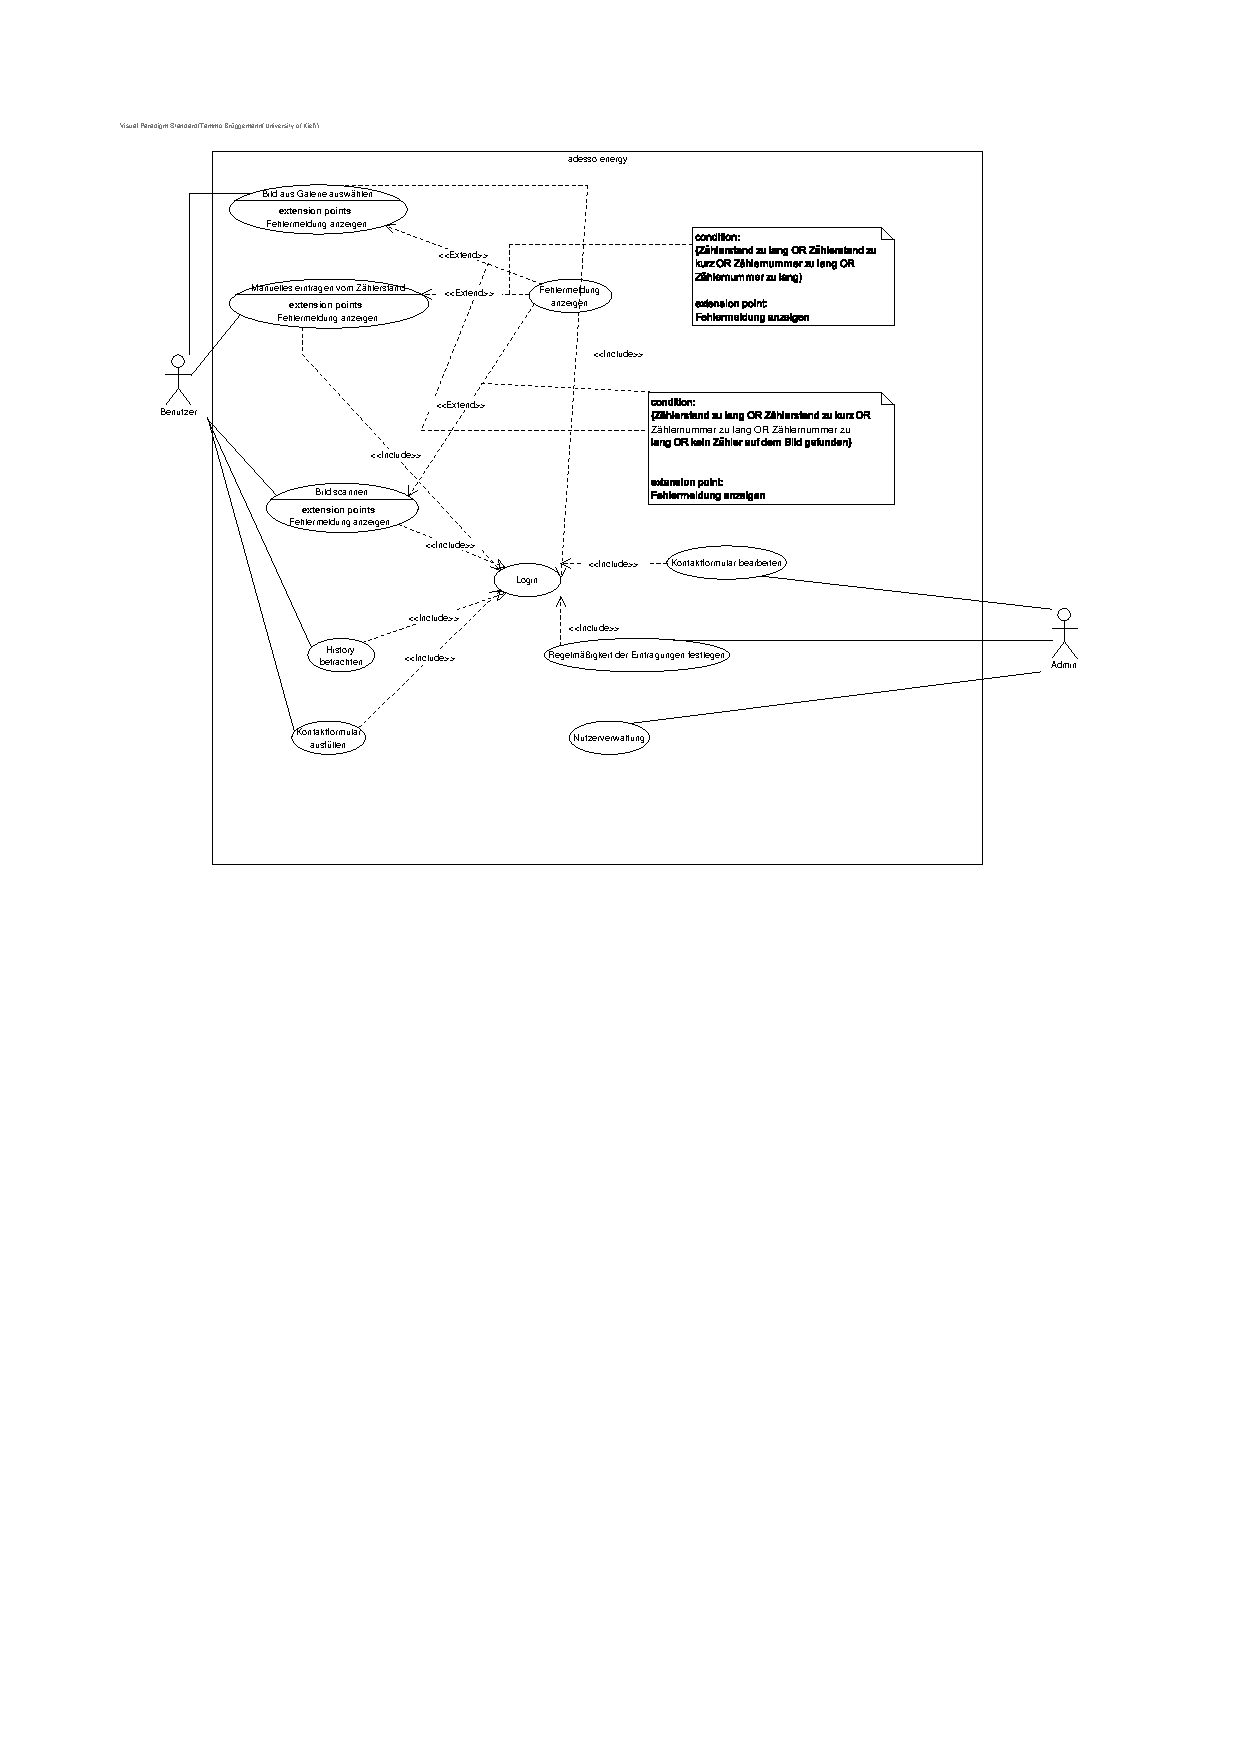
\includegraphics[width=20cm]{./img/mustCase}
%	\centering
%	\missingfigure{Anwendungsfalldiagramm - App}		
%	\caption{Anwendungsfalldiagramm - App}
%	\label{fig:anwendungsfalldiagramm-app}
\end{figure}

\newpage

\begin{figure}[h]
	\centering
	\begin{tabularx}{\textwidth}{ X | X }
		\textbf{Anwendungsfall ID} & 1 \\ \hline
		\textbf{Anwendungsfallname} & Bild hochladen  - Foto \\ \hline
		\textbf{Initiierender Akteur} & Benutzer \\ \hline
		\textbf{Weitere Akteure} & - \\ \hline
		\textbf{Kurzbeschreibung} & Der Benutzer macht in der App ein Foto und lädt dieses hoch.   \\ \hline
		\textbf{Vorbedingungen} & 
		\begin {itemize}
			\item Eingeloggt sein. 
			\item Hauptbildschirm geöffnet.
			\item Auf Kamera FAB gedrückt.
		\end{itemize} \\ \hline
		\textbf{Nachbedingungen} & Zählerstand wurde erkannt und eingetragen.  \\ \hline
		\textbf{Ablauf} &
		\begin{enumerate}
			\item Benutzer macht Foto.
			\item Benutzer bestätigt Senden des Fotos.
			\item Azure wertet Bild aus.
			\item Erkannte Zählernummer und Zählerstand werden angezeigt.
			\item Benutzer bestätigt Korrektheit der Zählernummer und des Zählerstandes.
		\end{enumerate} \\ \hline
		\textbf{Alternative} &
		\begin{enumerate}
			\item Benutzer macht Foto.
			\item Benutzer bestätigt Senden des Fotos.
			\item Azure wertet Bild aus.
			\item Erkannte Zählernummer und Zählerstand werden angezeigt.
			\item Benutzer bricht Aktion ab.
		\end{enumerate} \\ &
		\begin{enumerate}
			\item Benutzer macht Foto.
			\item Benutzer bestätigt Senden des Fotos.
			\item Azure wertet Bild aus.
			\item Erkannte Zählernummer und Zählerstand werden angezeigt.
			\item Benutzer verbessert Eingabe manuell.
		\end{enumerate} \\


	\end{tabularx}
\end{figure}

\begin{figure}[h]
	\centering
	\begin{tabularx}{\textwidth}{ X | X }
	 \hline
		\textbf{Ausnahme} &
		\begin{enumerate}
			\item Benutzer macht Foto.
			\item Benutzer bestätigt Senden des Fotos.
			\item Azure wertet Bild aus
			\item Fehler beim Auslesen der Zählernummer oder des Zählerstandes.
			\item $\lbrack$ Use-Case: Fehlermeldung wird angezeigt $\rbrack$
		\end{enumerate} \\ &
		\begin{enumerate}
			\item Benutzer macht Foto.
			\item Benutzer bestätigt Senden des Fotos.
			\item Azure wertet Bild aus
			\item Zählernummer und Zählerstand wurden erkannt, aber mindestens einer der beiden Werte ist unzulässig. (falsches Format)
			\item $\lbrack$ Use-Case: Fehlermeldung wird angezeigt $\rbrack$
		\end{enumerate} \\  &
		\begin{enumerate}
			\item Benutzer macht Foto.
			\item Benutzer bestätigt Senden des Fotos.
			\item Es liegt ein Serverfehler vor.
			\item Die App zeigt eine 'Bitte versuche es nochmal'-Meldung.
		\end{enumerate} \\ \hline &
		\begin{enumerate}
			\item Benutzer macht Foto.
			\item Benutzer bestätigt Senden des Fotos.
			\item Nutzer hat keine Internetverbindung.
			\item Die App zeigt eine 'Du bist offline'-Meldung.
		\end{enumerate} \\ \hline
		\textbf{Benutzte Anwendungsfälle} & Fehlermeldung wird angezeigt \\ \hline
		\textbf{Spezielle Anforderungen} & - \\ \hline
		\textbf{Annahmen} & -
	\end{tabularx}
	\caption{Anwendungsfall Bildhochladen-1}
	\label{fig:anwendungsfall-server-tabelle-xx-1}
\end{figure}

\newpage

\begin{figure}[h]
	\centering
	\begin{tabularx}{\textwidth}{ X | X }
		\textbf{Anwendungsfall ID} & 2 \\ \hline
		\textbf{Anwendungsfallname} & Zählerstand manuell eingeben. \\ \hline
		\textbf{Initiierender Akteur} & Benutzer \\ \hline
		\textbf{Weitere Akteure} & - \\ \hline
		\textbf{Kurzbeschreibung} & Der Benutzer hat, neben dem Abfotografieren des Zählerstandes, auch noch die Möglichkeit den Zählerstand manuell 									einzugeben.  \\ \hline
		\textbf{Vorbedingungen} & 
		\begin {itemize}
			\item Eingeloggt sein. 
			\item Hauptbildschirm geöffnet.
			\item Zähler auswählen.
			\item Auf Button 'Neue manuelle Eingabe' drücken.
		\end{itemize}\\ \hline
		\textbf{Nachbedingungen} & Zählerstand wurde eingetragen.  \\ \hline
		\textbf{Ablauf} &
		\begin{enumerate}
			\item Benutzer überprüft ob angezeigte Zählernummer mit der Zählernummer des ausgewählten Zählers übereinstimmt.
			\item Benutzer gibt Zählerstand ein.
			\item Benutzer bestätigt Zählerstand.
		\end{enumerate} \\ \hline
		\textbf{Alternative} & - \\ \hline
		\textbf{Ausnahme} &
		\begin{enumerate}
			\item Benutzer überprüft ob angezeigte Zählernummer mit der Zählernummer des ausgewählten Zählers übereinstimmt.
			\item Benutzer bricht Aktion ab.
		\end{enumerate}  \\  &
		\begin{enumerate}
			\item Benutzer überprüft ob angezeigte Zählernummer mit der Zählernummer des ausgewählten Zählers übereinstimmt.
			\item Benutzer gibt Zählerstand ein.
			\item Benutzer bestätigt Zählerstand.
			\item Zählerstand ist unzulässig. (falsches Format)
			\item 'Dieser Wert ist unzulässig. Bitte erneut eingeben'-Meldung wird angezeigt. 
		\end{enumerate} \\


	\end{tabularx}
\end{figure}

\begin{figure}[h]
	\centering
	\begin{tabularx}{\textwidth}{ X | X }
	&
		\begin{enumerate}
			\item Benutzer überprüft ob angezeigte Zählernummer mit der Zählernummer des ausgewählten Zählers übereinstimmt.
			\item Benutzer gibt Zählerstand ein.
			\item Benutzer bestätigt Zählerstand.
			\item Es liegt ein Serverfehler vor.
			\item Die App zeigt eine 'Bitte versuche es nochmal'-Meldung. 
		\end{enumerate} \\  &
		\begin{enumerate}
			\item Benutzer überprüft ob angezeigte Zählernummer mit der Zählernummer des ausgewählten Zählers übereinstimmt.
			\item Benutzer gibt Zählerstand ein.
			\item Benutzer bestätigt Zählerstand.
			\item Nutzer hat keine Internetverbindung.
			\item Die App zeigt eine 'Du bist offline'-Meldung.
		\end{enumerate}  \\ \hline
		\textbf{Benutzte Anwendungsfälle} & - \\ \hline
		\textbf{Spezielle Anforderungen} & - \\ \hline
		\textbf{Annahmen} & -
	\end{tabularx}
	\caption{Zählerstand manuell eingeben.}
	\label{fig:anwendungsfall-server-tabelle-xx-1}
\end{figure}

\newpage

\begin{figure}[h]
	\centering
	\begin{tabularx}{\textwidth}{ X | X }
		\textbf{Anwendungsfall ID} & 3 \\ \hline
		\textbf{Anwendungsfallname} & Fehlermeldung anzeigen. \\ \hline
		\textbf{Initiierender Akteur} & Benutzer \\ \hline
		\textbf{Weitere Akteure} & - \\ \hline
		\textbf{Kurzbeschreibung} & Falls beim Auslesen eines Bildes ein Problem auftritt, wird eine dem User eine Fehlermeldung angezeigt.   \\ \hline
		\textbf{Vorbedingungen} & 
		\begin {itemize}
			\item Eingeloggt sein. 
			\item Hauptbildschirm geöffnet.
			\item Bild wurde hochgeladen.
			\item Azure konnte Bild nicht auswerten.
		\end{itemize}\\ \hline
		\textbf{Nachbedingungen} & - \\ \hline
		\textbf{Ablauf} &
		\begin{enumerate}
			\item Meldung 'Scan nicht erfolgreich' wird angezeigt
			\item Benutzer drückt auf 'Neuer Scan"
			\item $\lbrack$ Use-Case: Bild hochladen - Foto $\rbrack$
		\end{enumerate} \\ \hline
		\textbf{Alternative} & 
		\begin{enumerate}
			\item Meldung 'Scan nicht erfolgreich' wird angezeigt
			\item Benutzer drückt auf 'Abbrechen'
			\item Benutzer ist wieder auf Startbildschirm
		\end{enumerate} \\ \hline
		\textbf{Ausnahme} & -   \\ \hline
		\textbf{Benutzte Anwendungsfälle} & Bild hochladen - Foto \\ \hline
		\textbf{Spezielle Anforderungen} & - \\ \hline
		\textbf{Annahmen} & -
	\end{tabularx}
	\caption{Fehlermeldung anzeigen.}
	\label{fig:anwendungsfall-server-tabelle-xx-1}
\end{figure}



